\section{Large-Scale Data Analysis}\label{experiments}

With our methodology on speed estimates, we next explain our findings on correlations between user mobility and mobile data access patterns in this section. We start with the correlation of the speed and the average mobile data access volumes. Then we reveal the relation of speed and average time intervals between consecutive mobile data accesses. Finally, we illustrate the correlation between speed and the types of app usage that are responsible for generating the corresponding mobile data traffic.

% \subsection{Dataset and Experimental Setup}

\change{(R1-4) We implement our speed estimation algorithm and mobile data usage pattern analysis algorithm in Python. We use the Voronoi package from Scipy ~\cite{scipy} to construct Voronoi maps with tower coordinates and Shapely ~\cite{shapely} for geometry calculations. All analysis is carried out on a single Cloudlab ~\cite{RicciEide:login14} c8220 server with two 10-core 2.2GHz E5-2660 processors and 256GB memory.}


\subsection{Speed and Data Volumes}

To estimate the speed, our algorithm requires a user has visited at least 3 towers consecutively. In the dataset, we find that around 13 million records out of 58 million records can be utilized. Although the dataset contains both user initiated network access and background network access, we find it very hard to separate them reliably. In our experiments, to balance the accuracy of speed estimates and the number of mobile data access records that have qualified speed estimates, we set the threshold of both distance ratio $d_{ratio}$ and duration ratio $\Delta t_{ratio}$ empirically as 0.6. After the filtering, we have around 1 million records out of total 13 million records that meet both criteria. \autoref{fig:speed_cdf} shows the cumulative density function (CDF) of both raw speed estimates without filtering and filtered speed estimates. As we can see that the filtered speed estimates are more realistic compared to raw speed estimates. Most of the false high speed estimates and low speed estimates are filtered out by setting thresholds of confidence levels for distance estimates and travel time estimates.
In the following experiments, we only show results in the speed range from 0 km/h to 100 km/h, since there are very few records with a speed estimate above 100 km/h for any meaningful insights.

\begin{figure}[h]
\centering
\subfigure[Empirical CDF of speed estimates.\label{fig:speed_cdf}]{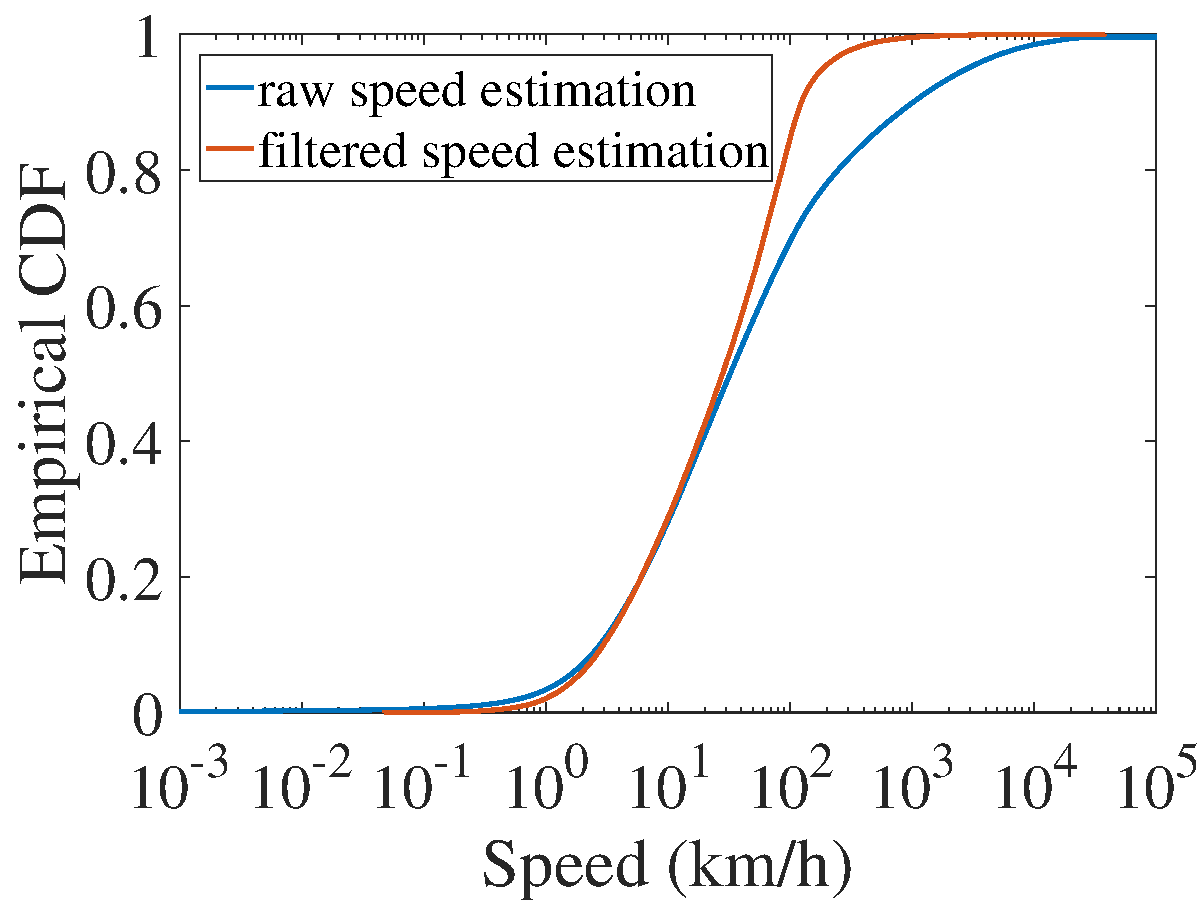
\includegraphics[width=0.45\linewidth]{./figures/speed_cdf.pdf}}
\subfigure[Correlation of speed estimates with data volumes.\label{fig:speed_vol}]{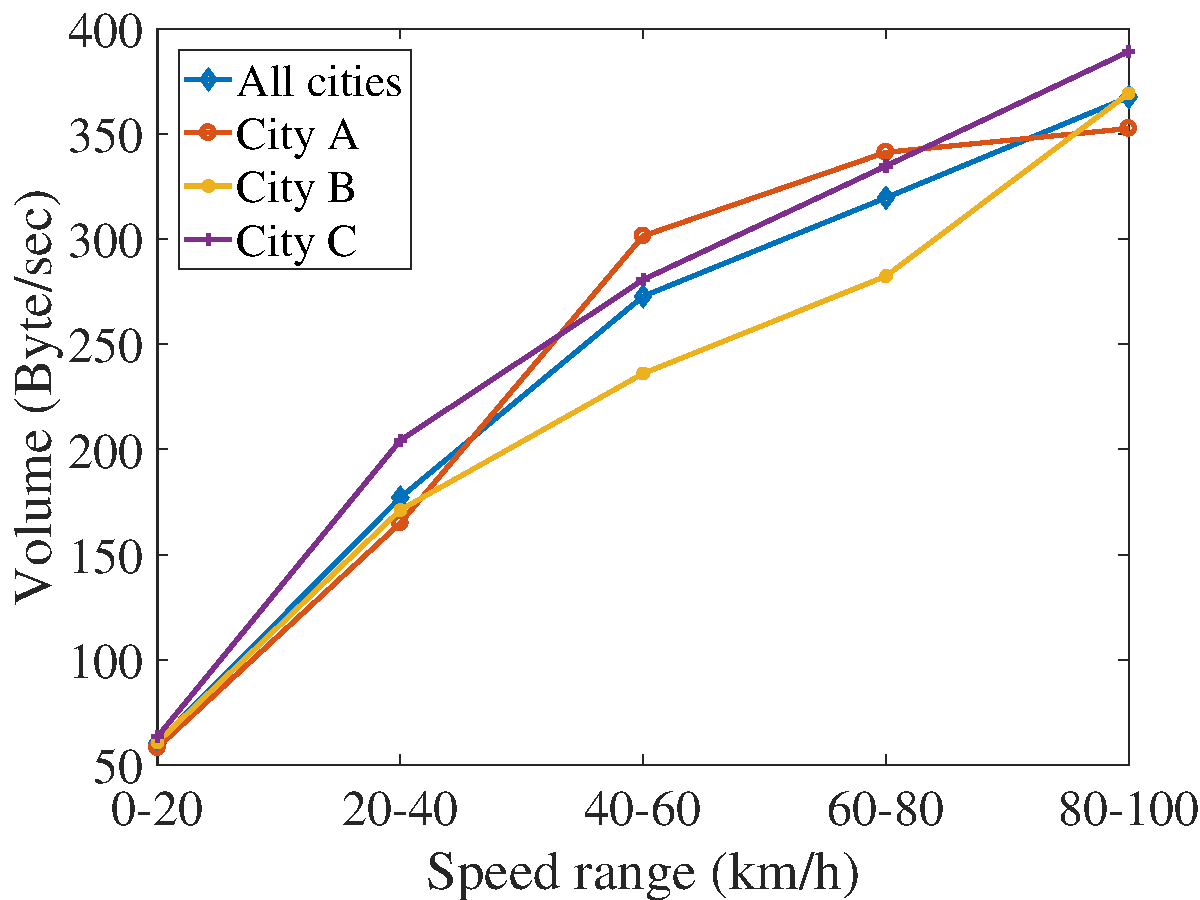
\includegraphics[width=0.45\linewidth]{./figures/large_font/speed_vol.pdf}}
\end{figure}

\begin{comment}
\begin{figure}[h]
    \centering
    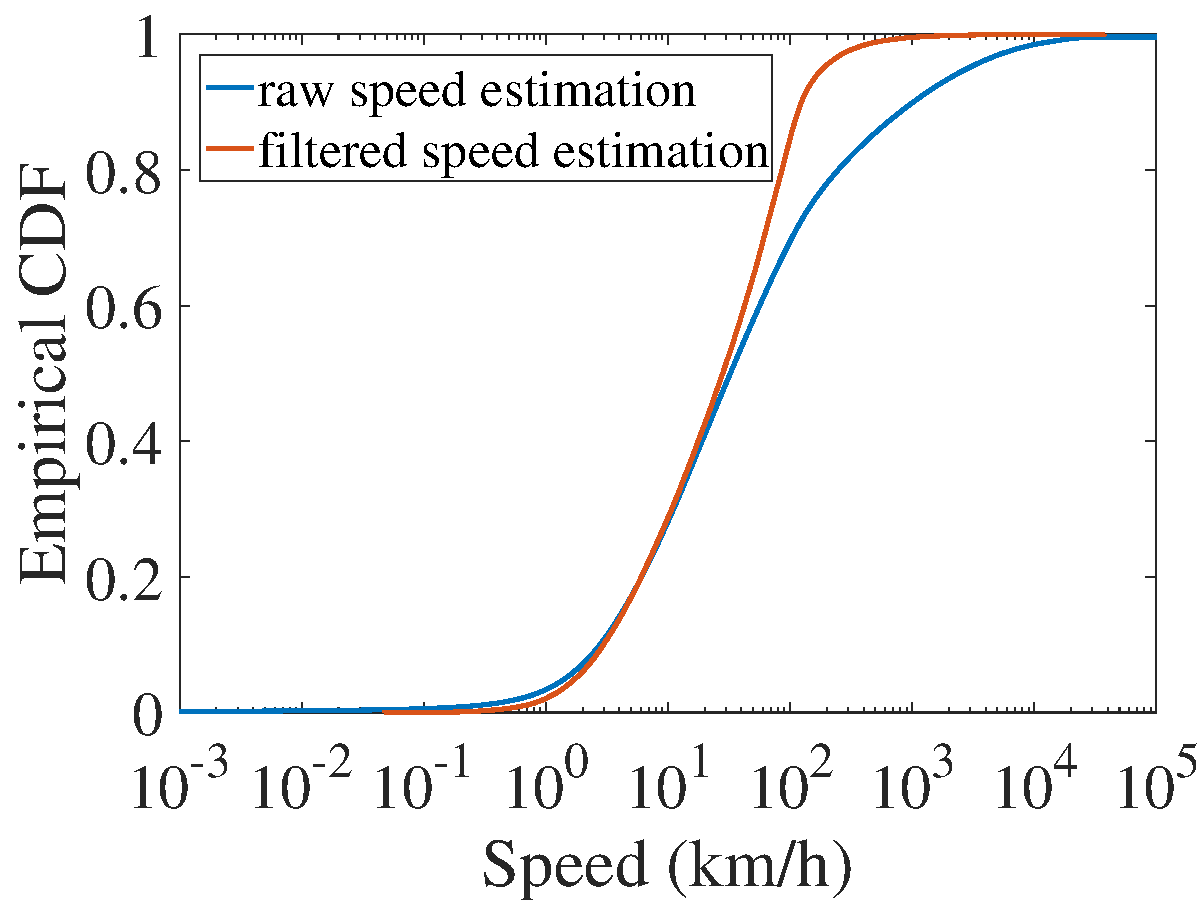
\includegraphics[width=0.5\linewidth]{./figures/speed_cdf.pdf}
    \caption{Empirical CDF of speed estimates.}
    \label{fig:speed_cdf}
\end{figure}

\begin{figure}[h]
    \centering
    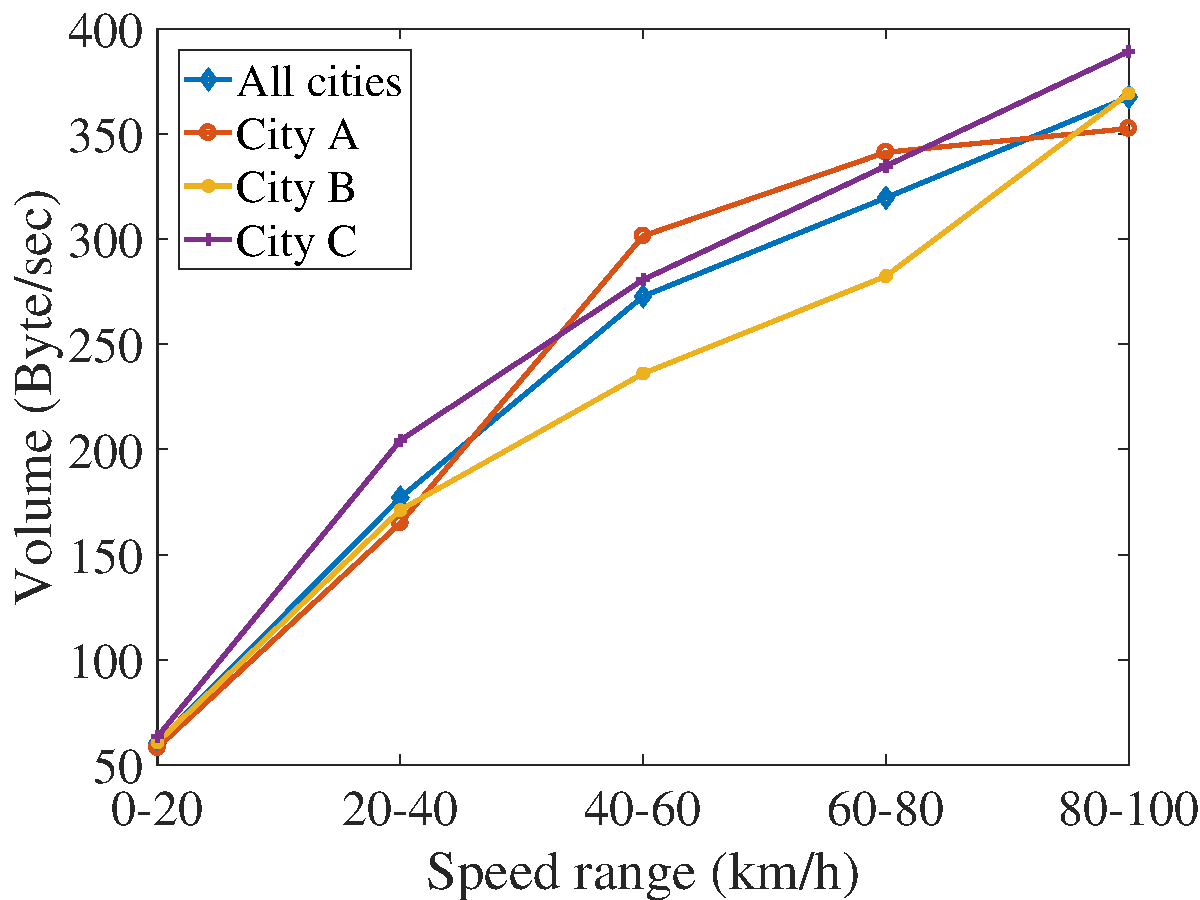
\includegraphics[width=0.5\linewidth]{./figures/large_font/speed_vol.pdf}
    \caption{The correlation of speed estimates with data volumes.}
    \label{fig:speed_vol}
\end{figure}
\end{comment}

\autoref{fig:speed_vol} shows the results of the correlation of user speed and the average mobile data access volumes per user per second. We demonstrate the data from all three cities combined and each city respectively. The figure shows a clear trend that users are more active in accessing mobile data as the speed increases and the trend holds true for all three cities. In fact, a user with speed estimates of 80-100 km/h could reach an average data volume of 6 times of a low-speed user. Similarly, this trend also holds true for all the cities. Note that these results only show an increase in the mobile data access volume as user speed increases. It does not suggest lower speed users access online contents less frequently. Actually, we believe one reason might be that a large portion of a low-speed user's online needs is already fulfilled by various kind of high-speed connections such as Wifi hotspots. To this end, we reach similar findings with previous work~\cite{yang2015characterizing} on the correlation of user mobility and mobile data access volume, except that the previous work used the number of towers visited by a user as the indicator of user mobility.

\subsection{Speed and Access Frequency}

\begin{figure}[h]
\centering
\subfigure[Average Time Interval\label{fig:speed_gap}]{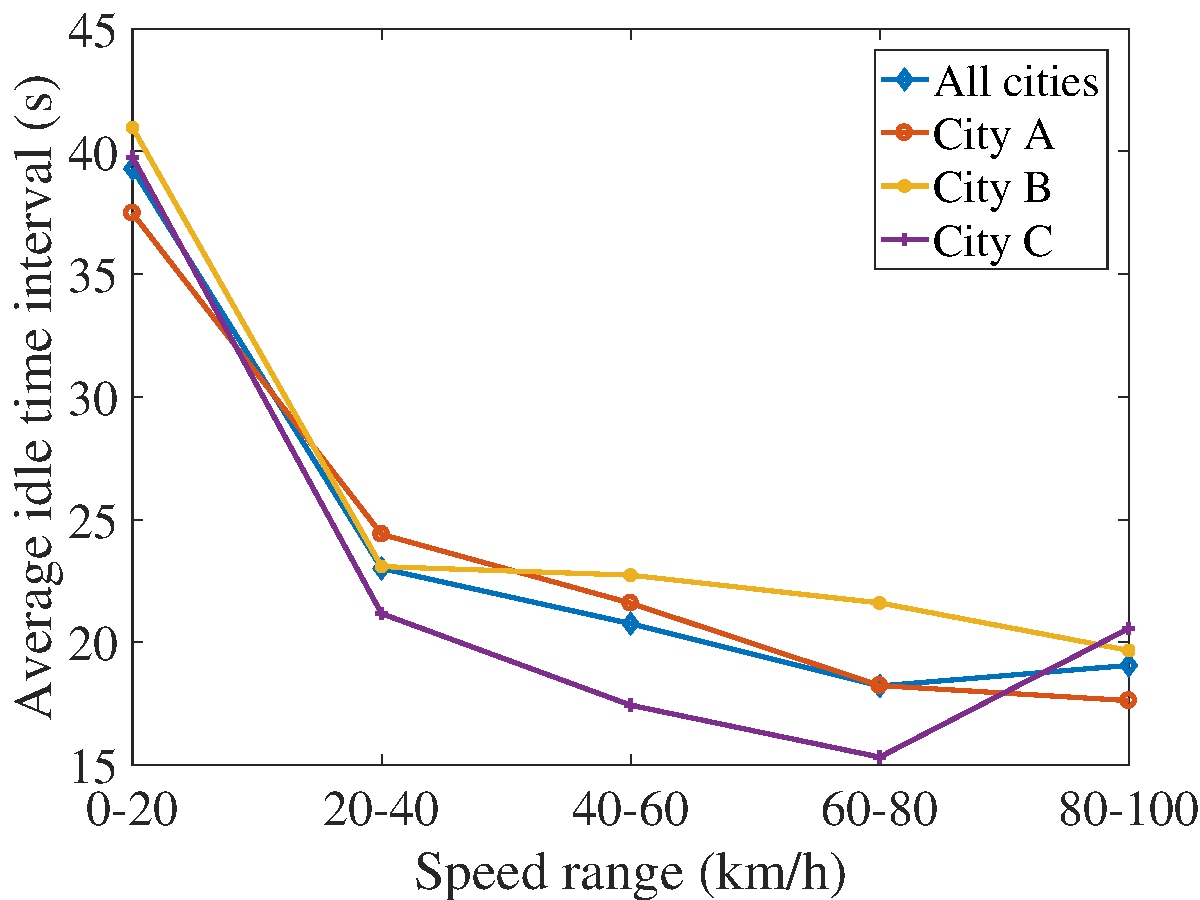
\includegraphics[width=0.32\linewidth]{./figures/large_font/speed_gap.pdf}}
\subfigure[Time Interval Empirical CDF\label{fig:speed_gap_cdf}]{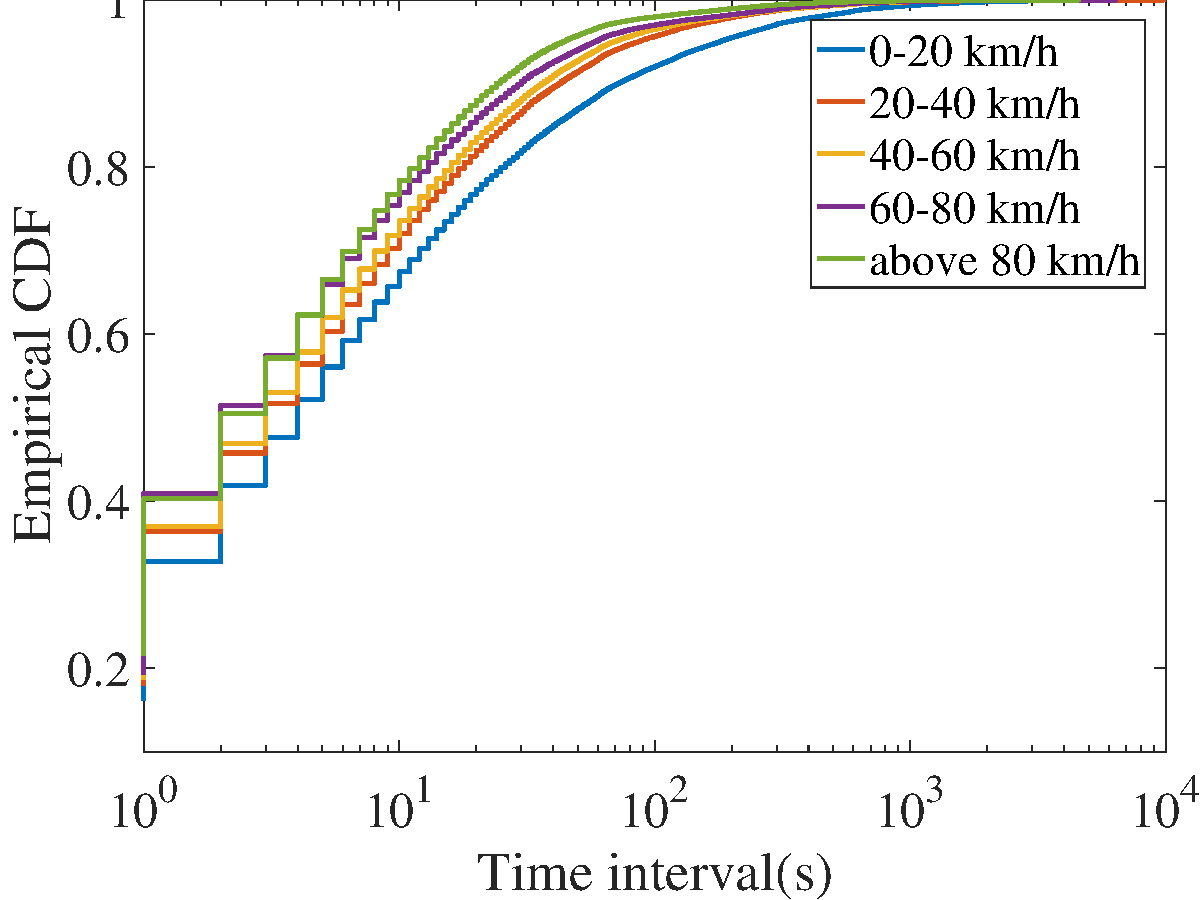
\includegraphics[width=0.31\linewidth]{./figures/large_font/speed_gap_cdf.pdf}}
\subfigure[Average Volume per Data Access\label{fig:speed_per_conn_vol}]{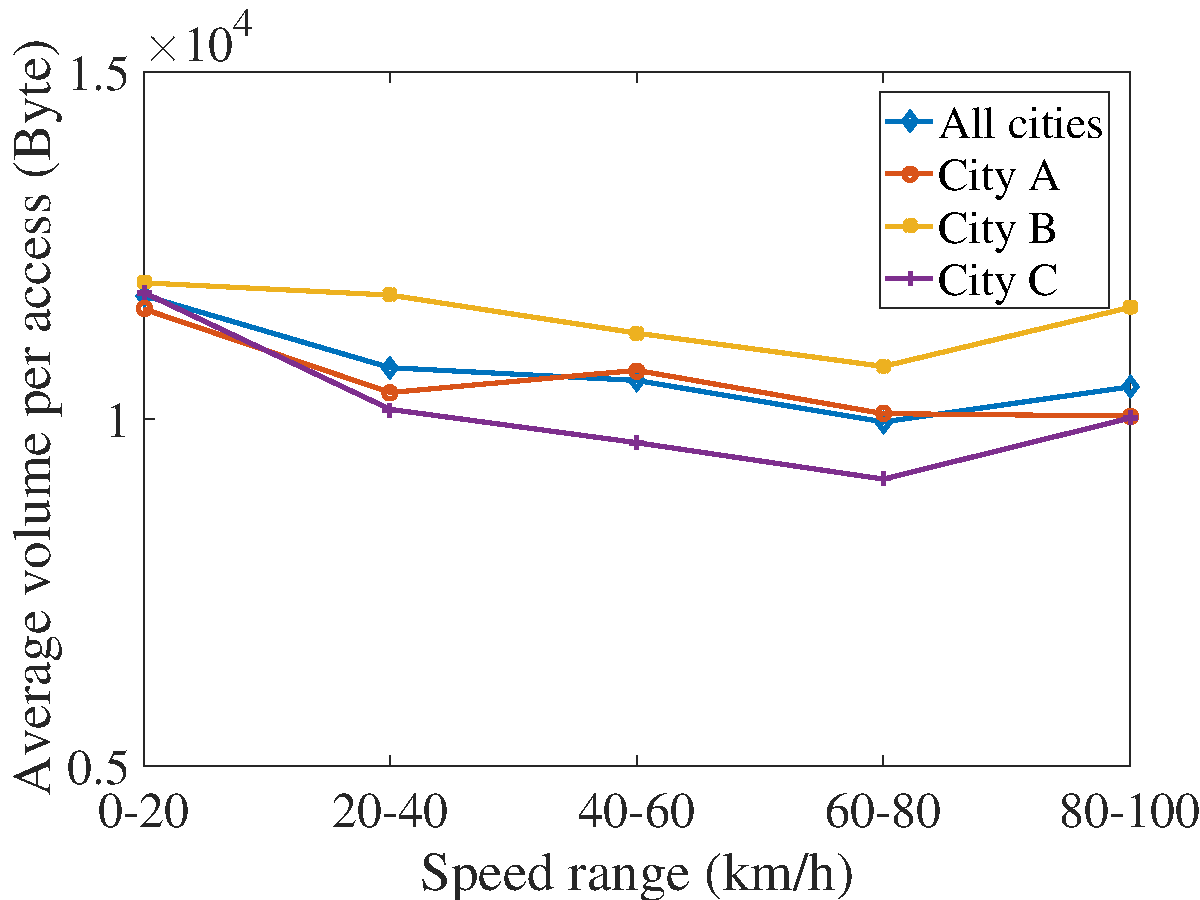
\includegraphics[width=0.328\linewidth]{./figures/large_font/speed_per_conn_vol.pdf}}
\caption{The correlation of speed estimates with (a) average idle time interval between consecutive data access, (b) idle time interval between consecutive connections, (c) average data access volume for each data access.}
\label{fig:speed_corr}
\end{figure}

\autoref{fig:speed_gap} shows the correlation of speed and average idle time intervals between consecutive mobile data access records. \change{Here a mobile data access record is defined as a single record entry in our dataset.} The CDF of data time intervals for various speed ranges of all three cities are also shown in \autoref{fig:speed_gap_cdf}. Note that since the time precision of our data trace is seconds, so there are steps in \autoref{fig:speed_gap_cdf}. The decrease in time intervals as speed increases suggests that high-speed user accesses mobile data more frequently than low-speed users. A user with a speed estimate of 80-100 km/h access mobile data almost twice more frequently than a user with a speed estimate of 0-20 km/h on average. The trend holds for all three cities except that there is an odd point at 80-100 km/h for one city, which may be caused by the lacking of available data.

We show the average volume for each data access in \autoref{fig:speed_per_conn_vol}. As the user speed increases, there is no apparent correlation with average volume for each data access. This suggests that increasing in the average volume which is shown in \autoref{fig:speed_vol} is mainly cause by the increased data access frequency, not the volume for each data access.

\subsection{Speed and App Usage}

According to the mobile service provider, each app in our dataset was assigned to one of 18 categories, as shown in \autoref{table:appcat}. 
%We first divided estimated user speed at 50km/h into two classes. The low speed class includes transportation modes such as walking, cycling, bus and other low speed vehicles. The high speed class includes mainly high speed vehicles.  
%We showed the number of data access per app category in \autoref{fig:speed_access_hl} and data volume per app category in \autoref{fig:speed_vol_hl}. In both figures, low speed users have more data access due to large user base. The share for each category holds similar trend for both high and low speed users. We will discuss more details on the contribution of each category to total data access in \autoref{fig:speed_appcat}.

\begin{table}[h]
	\centering
	\begin{tabular}{lrr}\hline
	App Category & \# Apps & Volume (GB) \\
    \hline
	Instant Messages & 30 & 97.3\\
	Reading & 101 & 17.6\\
	Microblog & 43 & 13.0\\
	Navigation  & 38 & 10.8\\
	Video  & 63 & 45.2\\
	Music  & 33 & 27.4\\
	App Market & 45 & 37.0\\
	Game  & 106 & 9.2\\
	Payment & 18 & 1.2\\
	Comic & 12 & 0.8\\
	Email & 10 & 1.5\\
	P2P & 8 & 3.9\\
	VOIP  & 17 & 0.3\\
	Multimedia Messages & 2 & 0.3\\
	Browsing & 558 & 353.5\\
	Finance  & 25 & 0.7\\
	Security  & 22 & 5.2\\
    Others  & 244 & 95.8\\
% 	Other1 & 237 & 74.7\\
% 	Other2 &   7 & 21.1\\
% 	Others & 464 & 118.9\\
    \hline
	\end{tabular}
	\caption{App categories}
	\label{table:appcat}
\end{table}

\begin{comment}
\begin{table}[h]
	\centering
	\begin{tabular}{lrrrr}\hline
    %             &         & \multicolumn{3}{c}{Volume (GB)} \\
	App Category & \# Apps & Total & Low Speed (filtered) & High Speed (filtered) \\
     &  & (GB) & (MB, $\le 50$ km/h) & (MB, $> 50$ km/h) \\
    \hline
	Instant Messages & 30 & 97.3 & 2040 & 409\\
	Reading & 101 & 17.6 & 371 & 72\\
	Microblog & 43 & 13.0 & 270 & 79\\
	Navigation  & 38 & 10.8 & 326 & 155\\
	Video  & 63 & 45.2 & \\
	Music  & 33 & 27.4\\
	App Market & 45 & 37.0\\
	Game  & 106 & 9.2\\
	Payment & 18 & 1.2\\
	Comic & 12 & 0.8\\
	Email & 10 & 1.5\\
	P2P & 8 & 3.9\\
	VOIP  & 17 & 0.3\\
	Multimedia Messages & 2 & 0.3\\
	Browsing & 558 & 353.5\\
	Finance  & 25 & 0.7\\
	Security  & 22 & 5.2\\
    Others  & 244 & 95.8\\
% 	Other1 & 237 & 74.7\\
% 	Other2 &   7 & 21.1\\
% 	Others & 464 & 118.9\\
    \hline
            &    &  &  100 & 100 \\
    \hline
	\end{tabular}
	\caption{App categories and data volume distribution}
	\label{table:appcat}
\end{table}
\end{comment}
\begin{comment}
\begin{figure}[h]
    \centering
    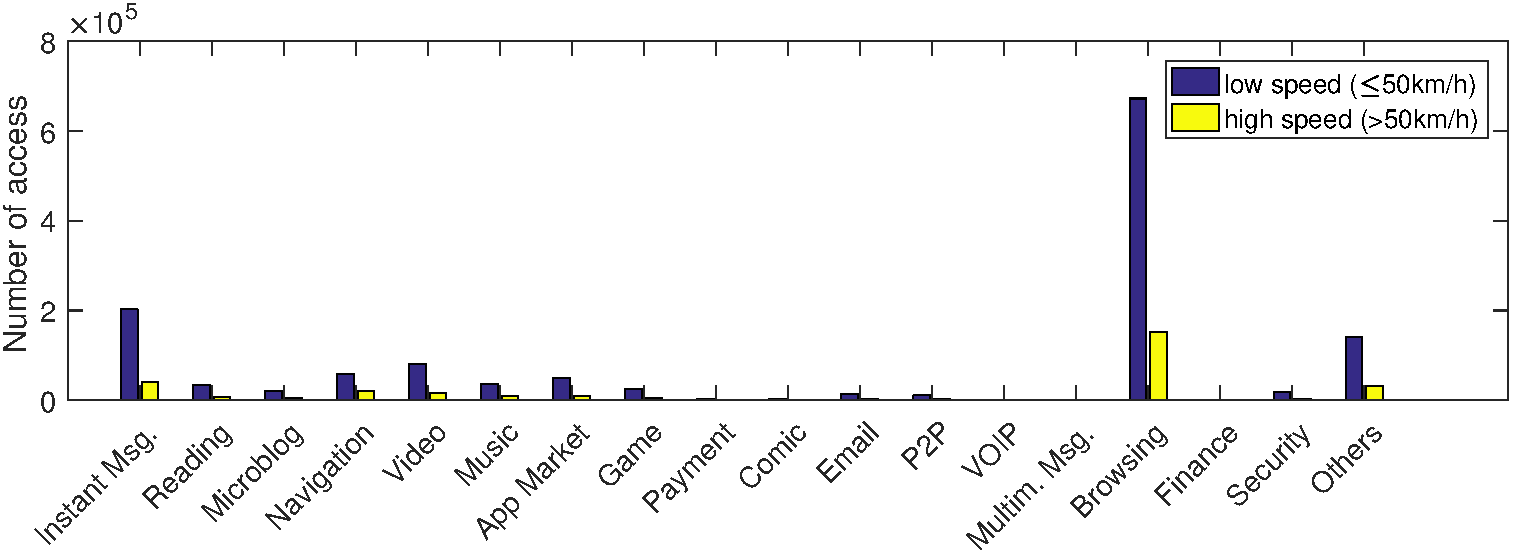
\includegraphics[width=\linewidth]{./figures/num_access_high_low_speed_8_6.pdf}
    \caption{The distribution of the number of access per app category with high and low speed users}
    \label{fig:speed_access_hl}
\end{figure}

\begin{figure}[h]
    \centering
    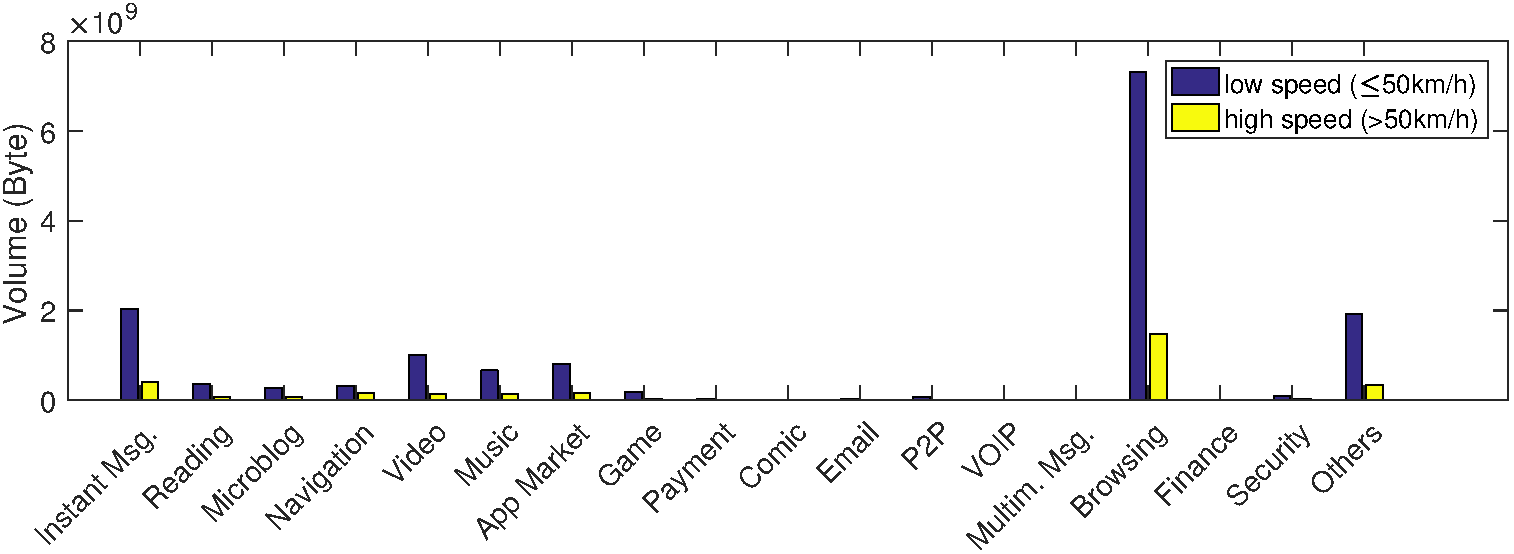
\includegraphics[width=\linewidth]{./figures/volume_high_low_speed_8_6.pdf}
    \caption{The distribution of data volume per app category with high and low speed users}
    \label{fig:speed_vol_hl}
\end{figure}
\end{comment}


\begin{figure}[h]
\centering
\subfigure[Number of unique apps used per minute\label{fig:app_per_min}]{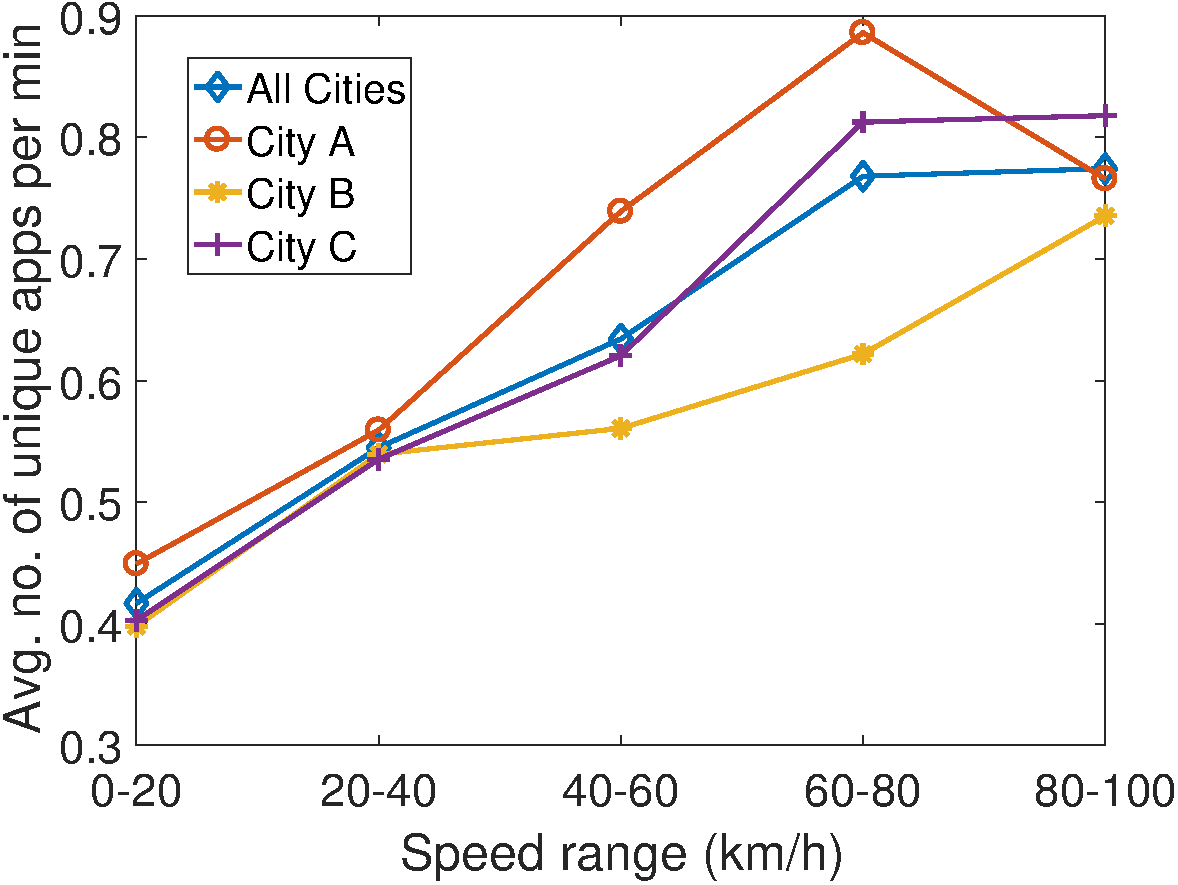
\includegraphics[width=0.32\linewidth]{./figures/app_per_min_8_6.pdf}}
\subfigure[App switch frequency\label{fig:switch_app}]{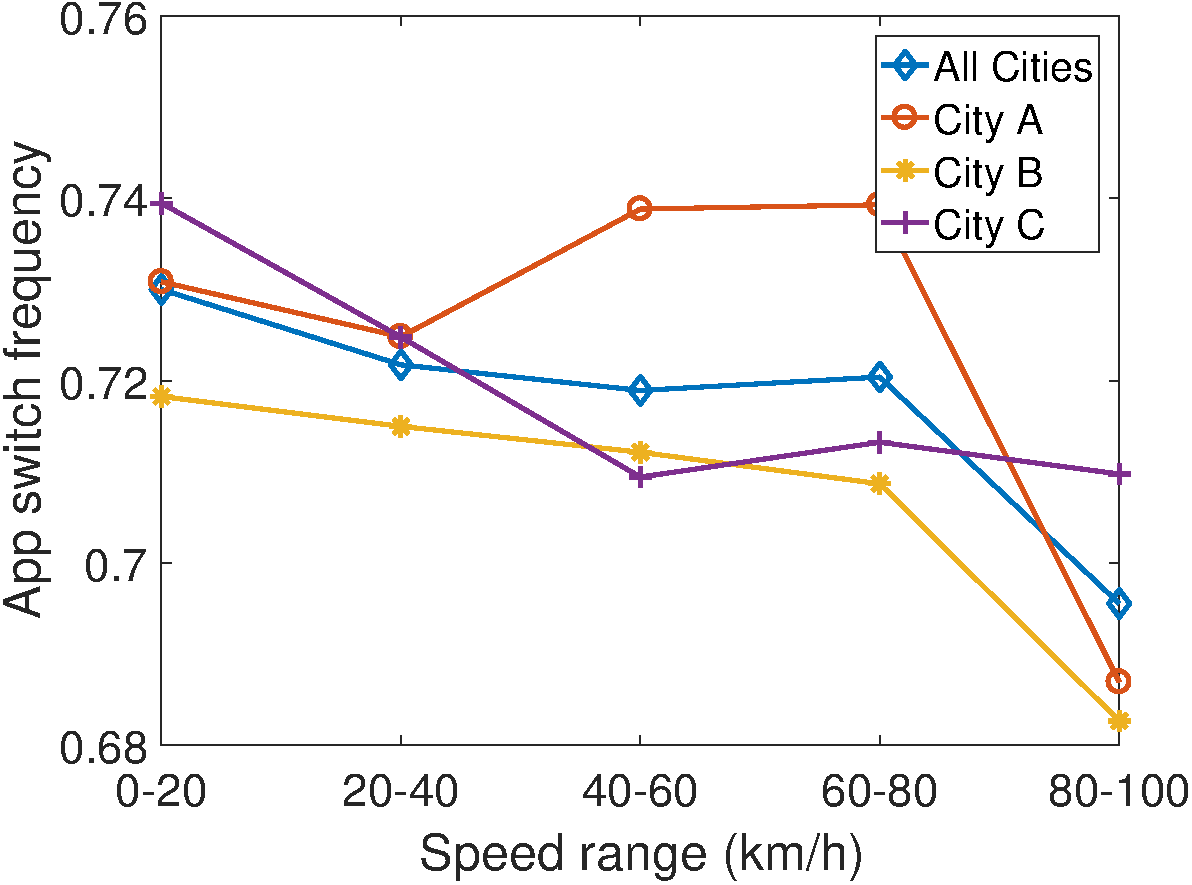
\includegraphics[width=0.32\linewidth]{./figures/app_switch_frequency_line_8_6.pdf}}
\subfigure[Average number of concurrently running apps\label{fig:app_overlap}]{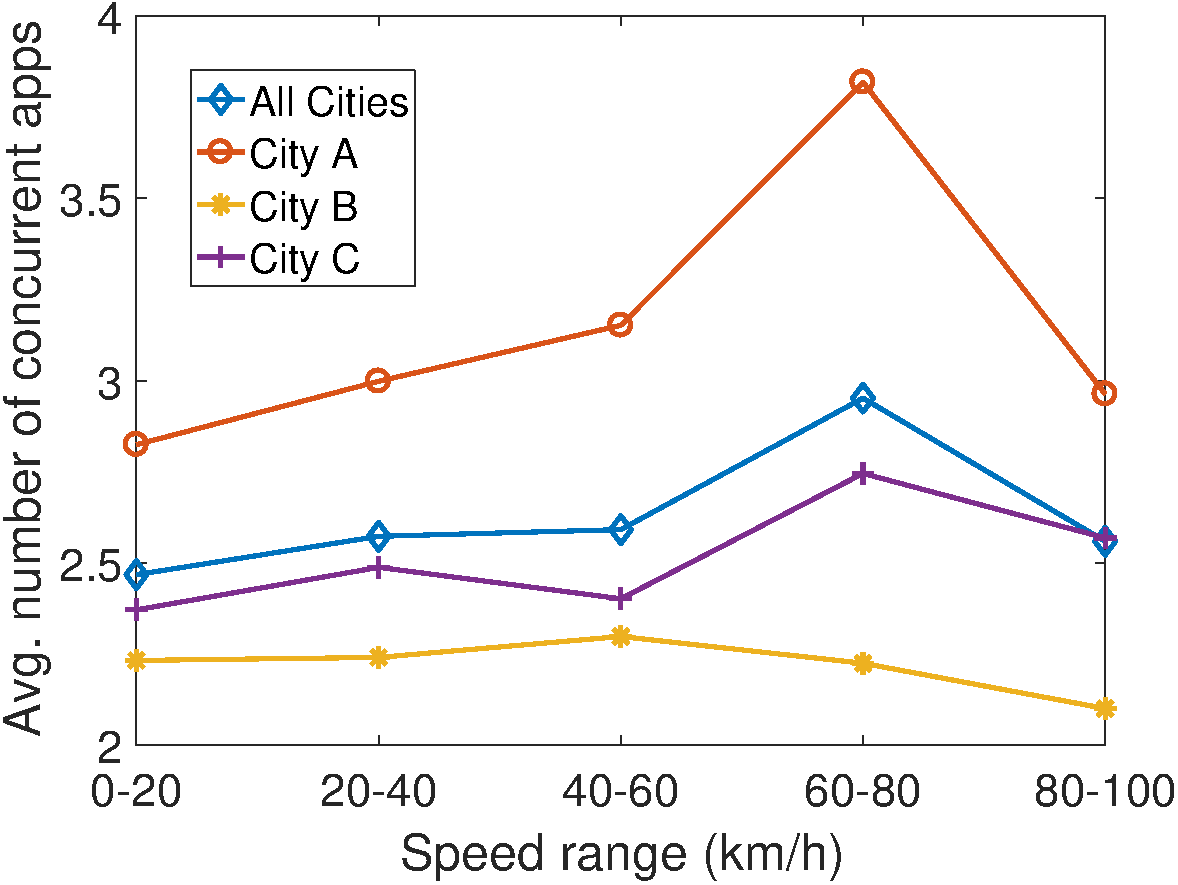
\includegraphics[width=0.32\linewidth]{./figures/app_overlap_8_6.pdf}}\\
\subfigure[Number of unique app categories used per minute\label{fig:app_cate_per_min}]{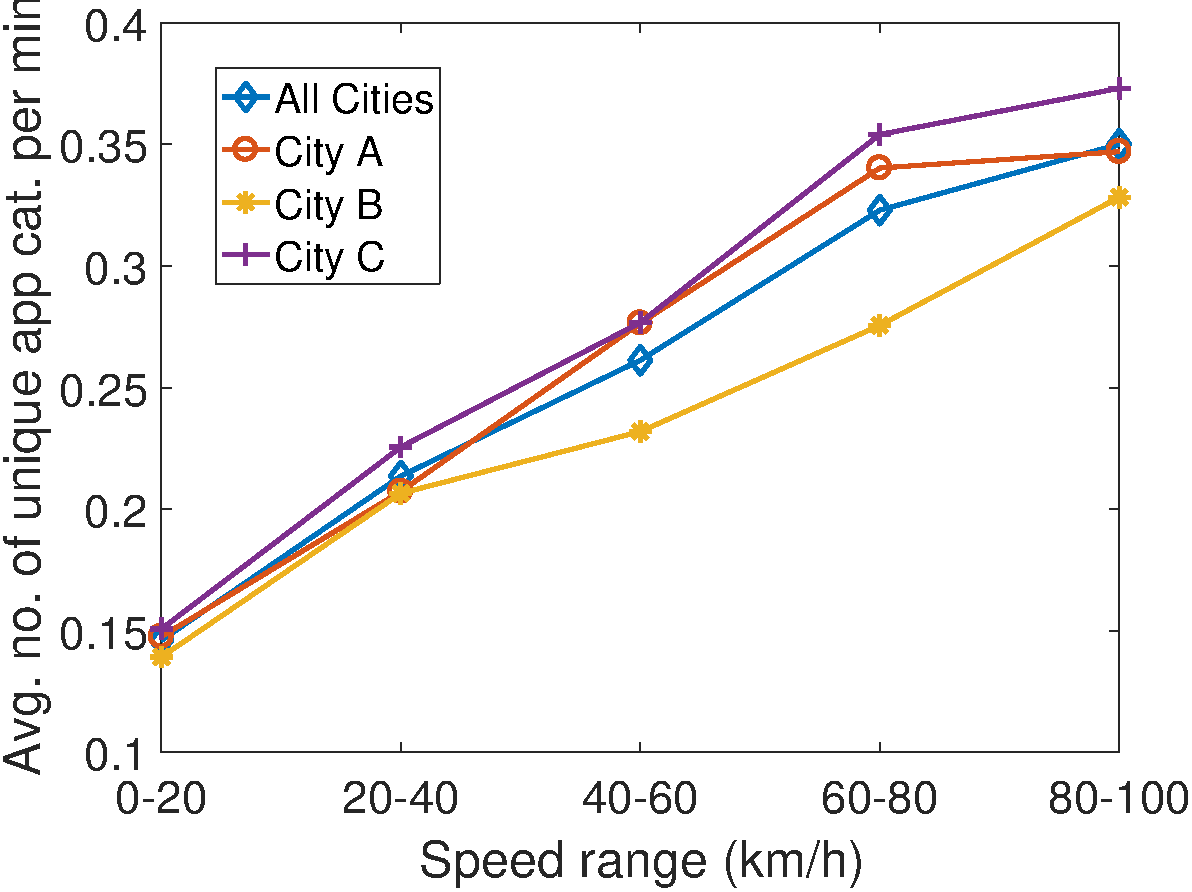
\includegraphics[width=0.32\linewidth]{./figures/app_category_per_min_8_6.pdf}}
\subfigure[App category switch frequency\label{fig:switch_app_category}]{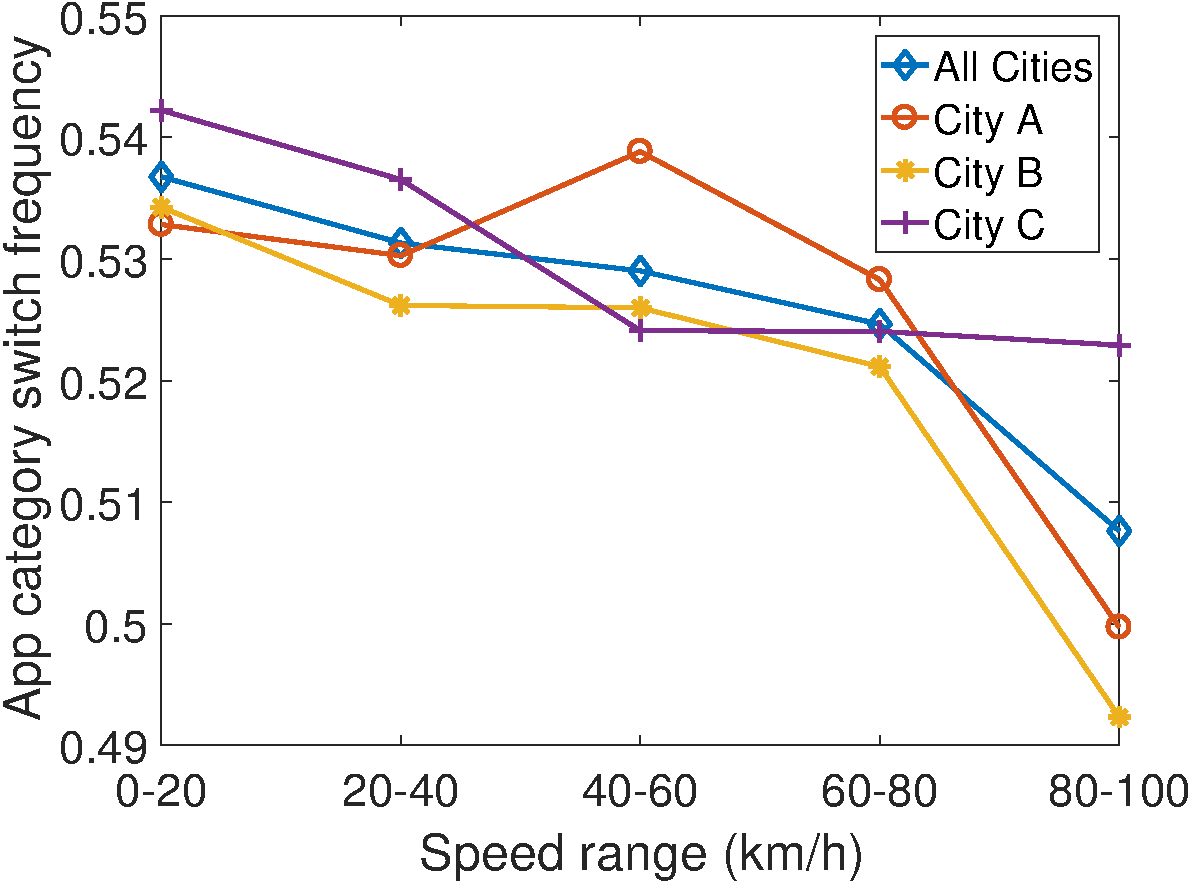
\includegraphics[width=0.32\linewidth]{./figures/app_category_switch_frequency_line_8_6.pdf}}
\subfigure[Average number of concurrently running app categories\label{fig:app_category_overlap}]{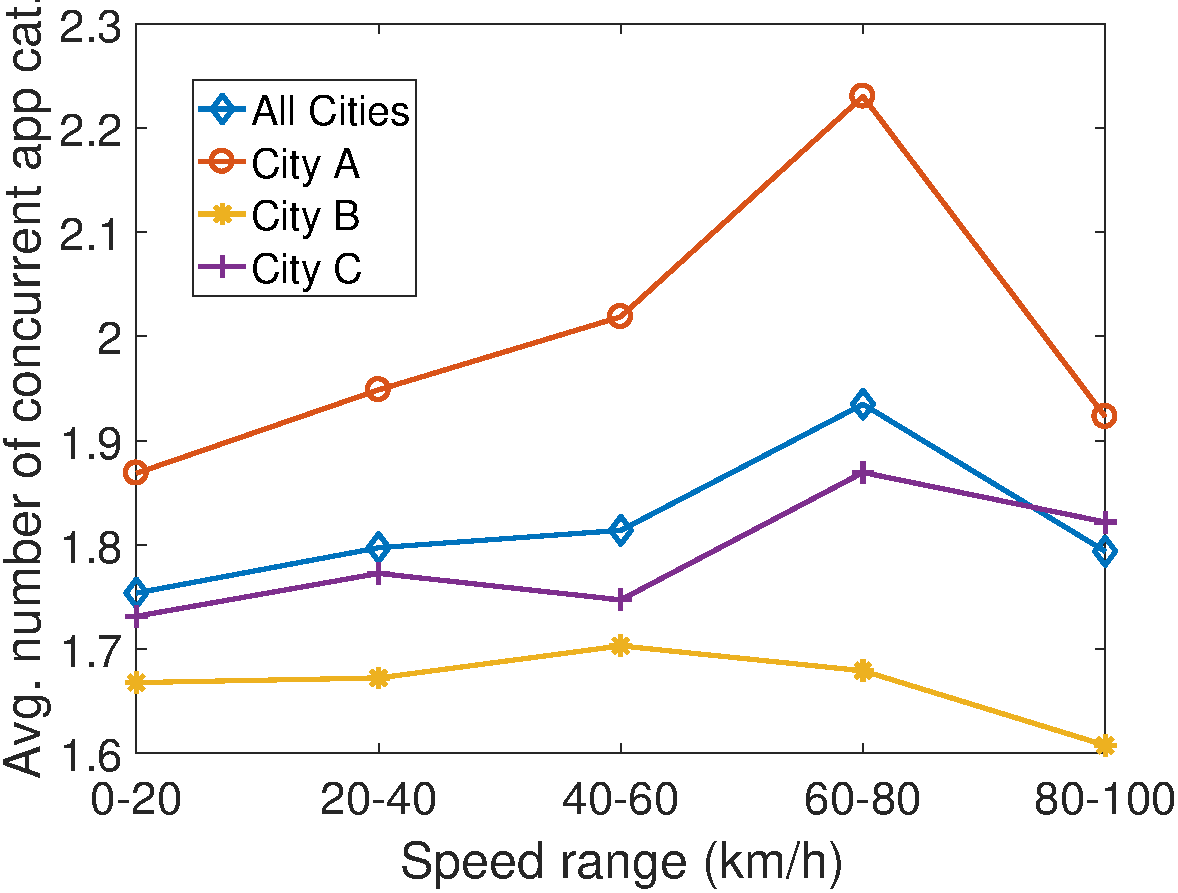
\includegraphics[width=0.32\linewidth]{./figures/app_category_overlap_8_6.pdf}}
\caption{Correlation of user speed and the number of unique apps and app categories used}
\end{figure}

\begin{comment}
\begin{figure}[h]
    \centering
		\subfigure[Number of unique apps used per minute\label{fig:app_per_min}]{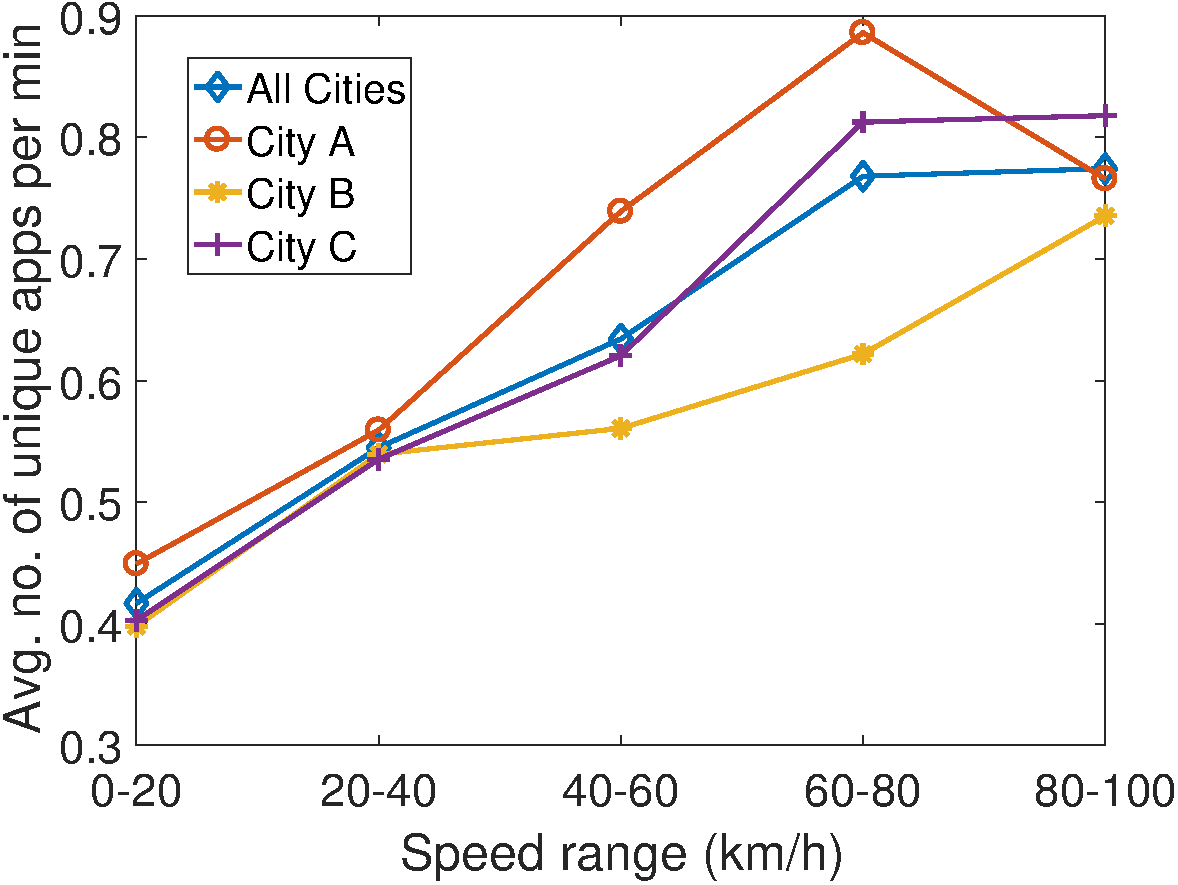
\includegraphics[width=0.48\linewidth]{./figures/app_per_min_8_6.pdf}}
		\subfigure[Number of unique app categories used per minute\label{fig:app_cate_per_min}]{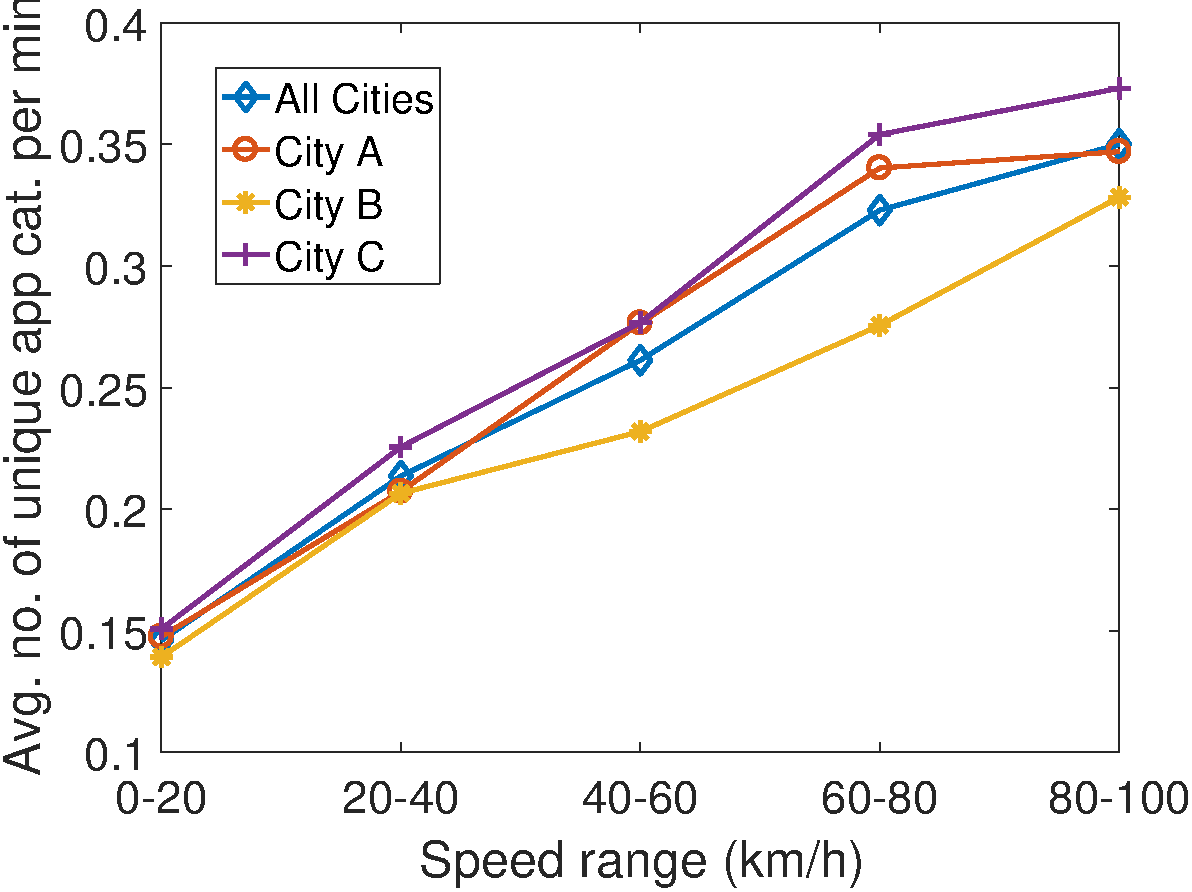
\includegraphics[width=0.48\linewidth]{./figures/app_category_per_min_8_6.pdf}}
    \caption{Correlation of user speed and the number of unique apps and app categories used}
    \label{fig:speed_app_used}
\end{figure}
\end{comment}

%In this section, we first show in
\autoref{fig:app_per_min} and \autoref{fig:app_cate_per_min} 
%\autoref{fig:speed_app_used} 
show the correlation between user speed and the average number of unique apps and app categories being used for each user during each data segment per minute.
The trend clearly shows that as the speed goes up, the app usage diversity increases rapidly.
A user with a speed estimate of 80-100 km/h could use as many as 2 times apps per unit of time compared to a low-speed user.
% This trend holds true for all the cities. 
An explanation might be that for users with high mobility, they may use their phones more often, use more kinds of apps, and be less likely to focus on one app for prolonged periods of time. 
% Both \autoref{fig:speed_app_used} and \autoref{fig:speed_app_switch} lead to the similar conclusion that unlike low speed users, users with high mobility may use their phones more often, switch between apps more, and be less likely to focus on one app for prolonged periods of time. 

\begin{comment}
\begin{figure*}
    \centering
		\subfigure[App switch frequency\label{fig:switch_app}]{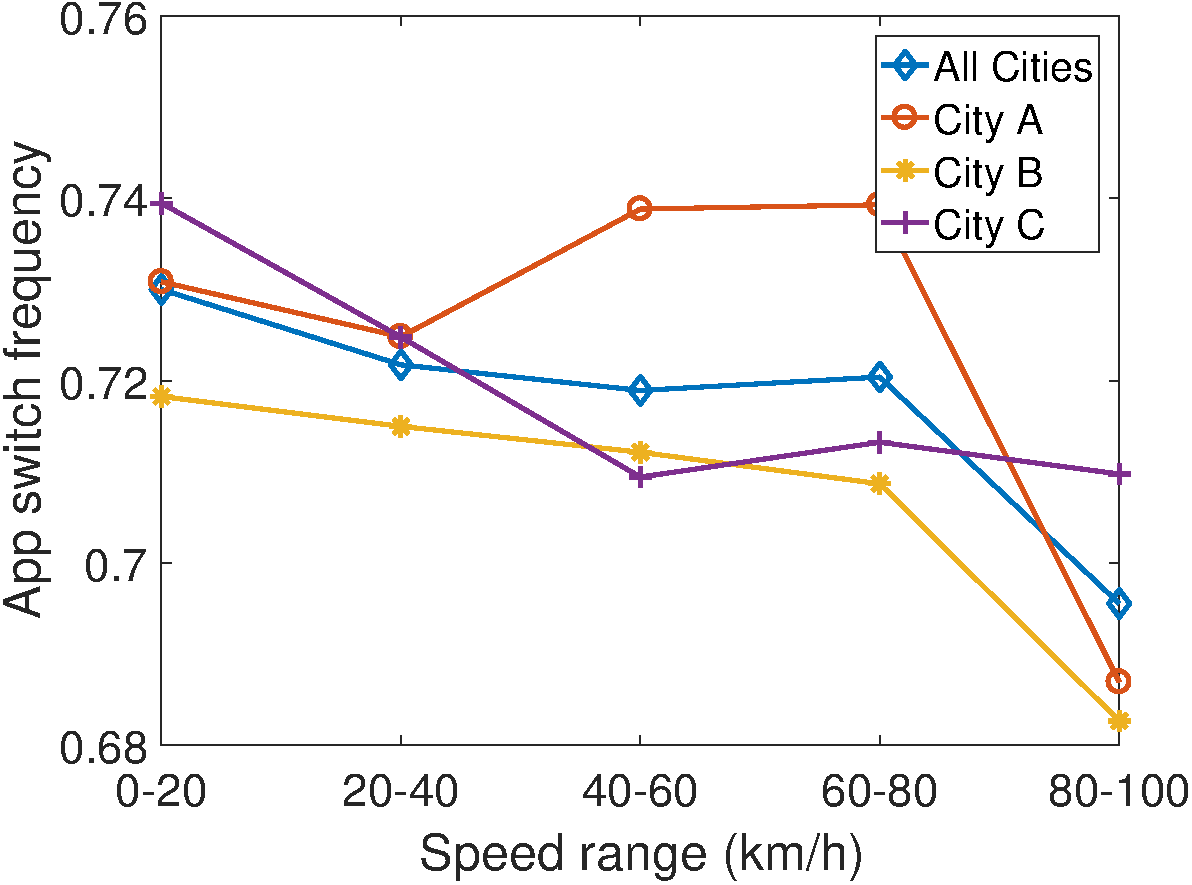
\includegraphics[width=0.48\linewidth]{./figures/app_switch_frequency_line_8_6.pdf}}
		\subfigure[App category switch frequency\label{fig:switch_app_category}]{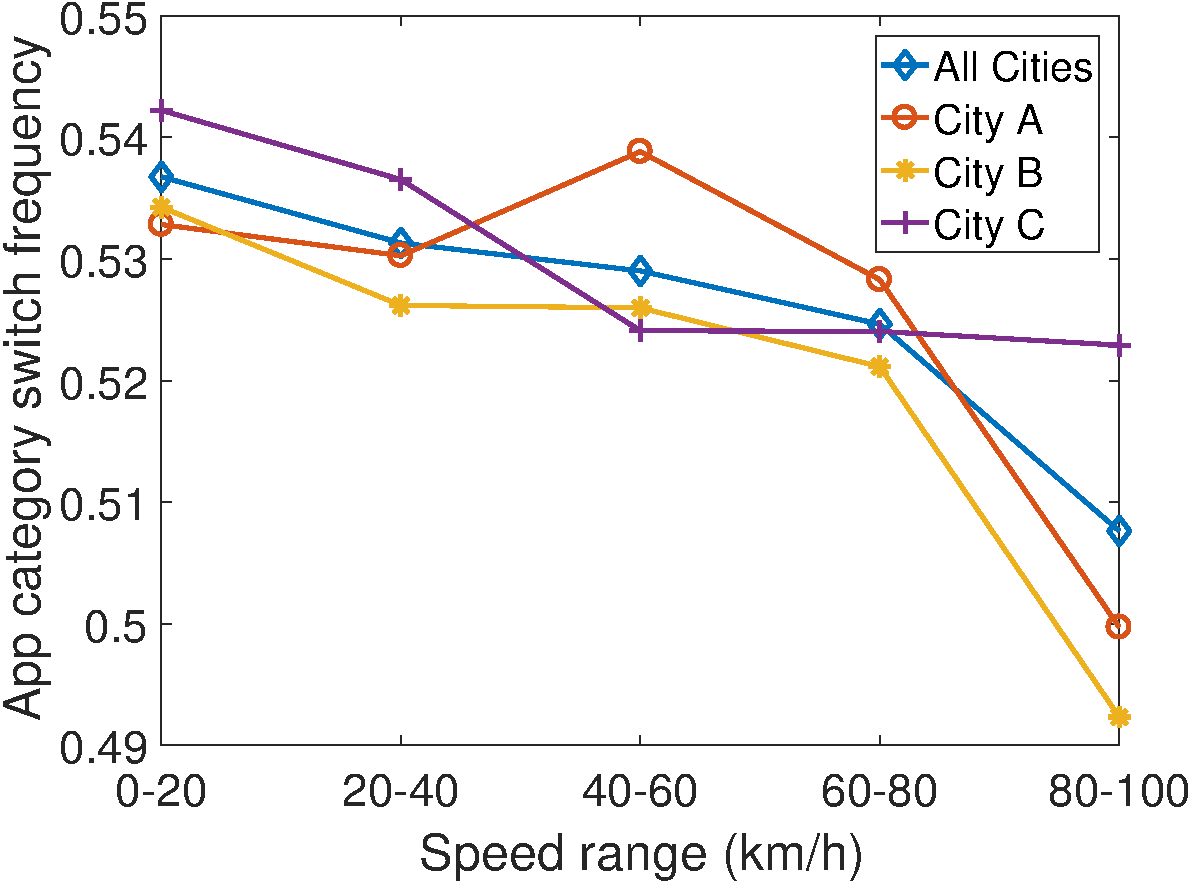
\includegraphics[width=0.48\linewidth]{./figures/app_category_switch_frequency_line_8_6.pdf}}
    \caption{Correlation of user speed and the frequencies of app and app category switch}
    \label{fig:speed_app_switch}
\end{figure*}
\end{comment}

In 
\autoref{fig:switch_app} and \autoref{fig:switch_app_category} 
%\autoref{fig:speed_app_switch}, 
we show the frequency of app switch and app category switch. They both follow the same trend that lower speed users tend to switch apps and app categories more frequently. Combined with 
\autoref{fig:app_per_min} and \autoref{fig:app_cate_per_min}, % \autoref{fig:speed_app_used}, 
we can see that although low speed users switch apps more frequently, they only switch among fewer number of apps.

\begin{comment}
\begin{figure*}
    \centering
		\subfigure[Average number of concurrently running apps\label{fig:app_overlap}]{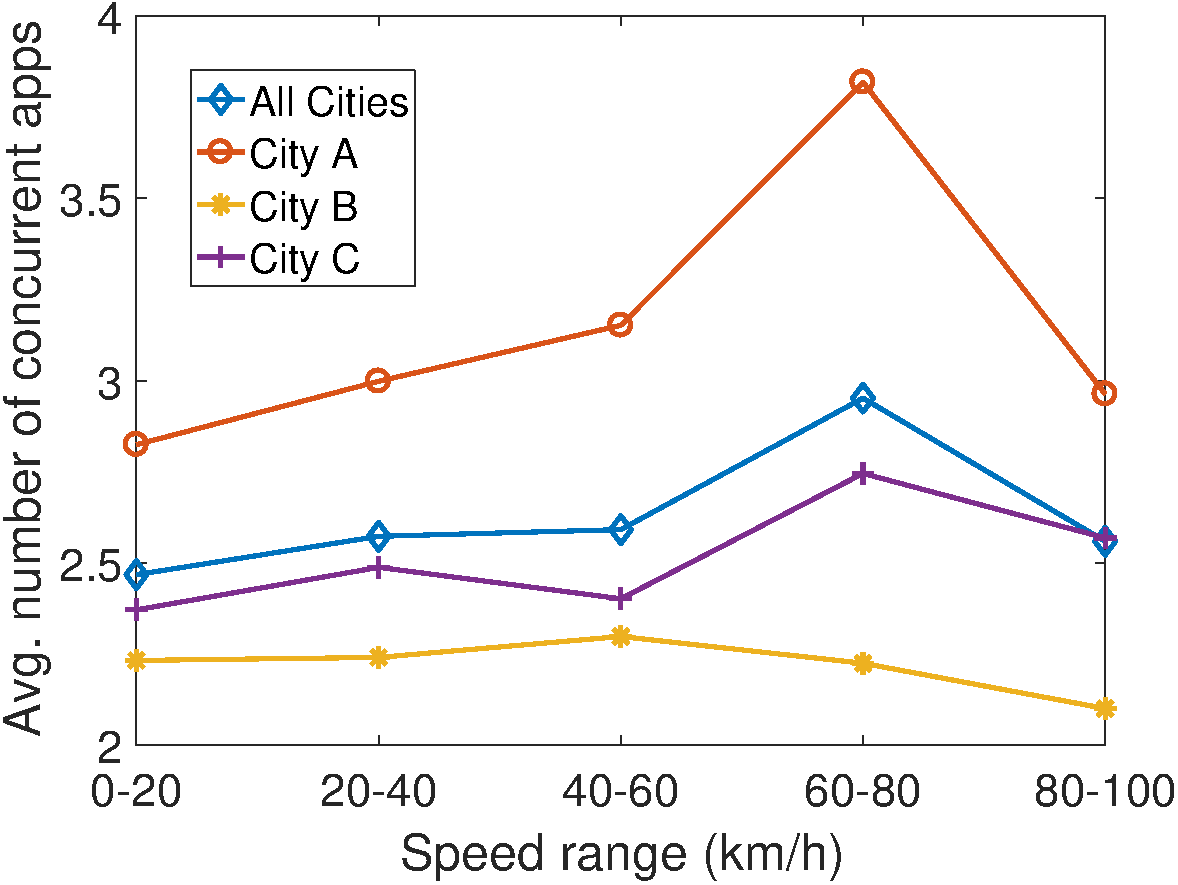
\includegraphics[width=0.48\linewidth]{./figures/app_overlap_8_6.pdf}}
		\subfigure[Average number of concurrently running app categories\label{fig:app_category_overlap}]{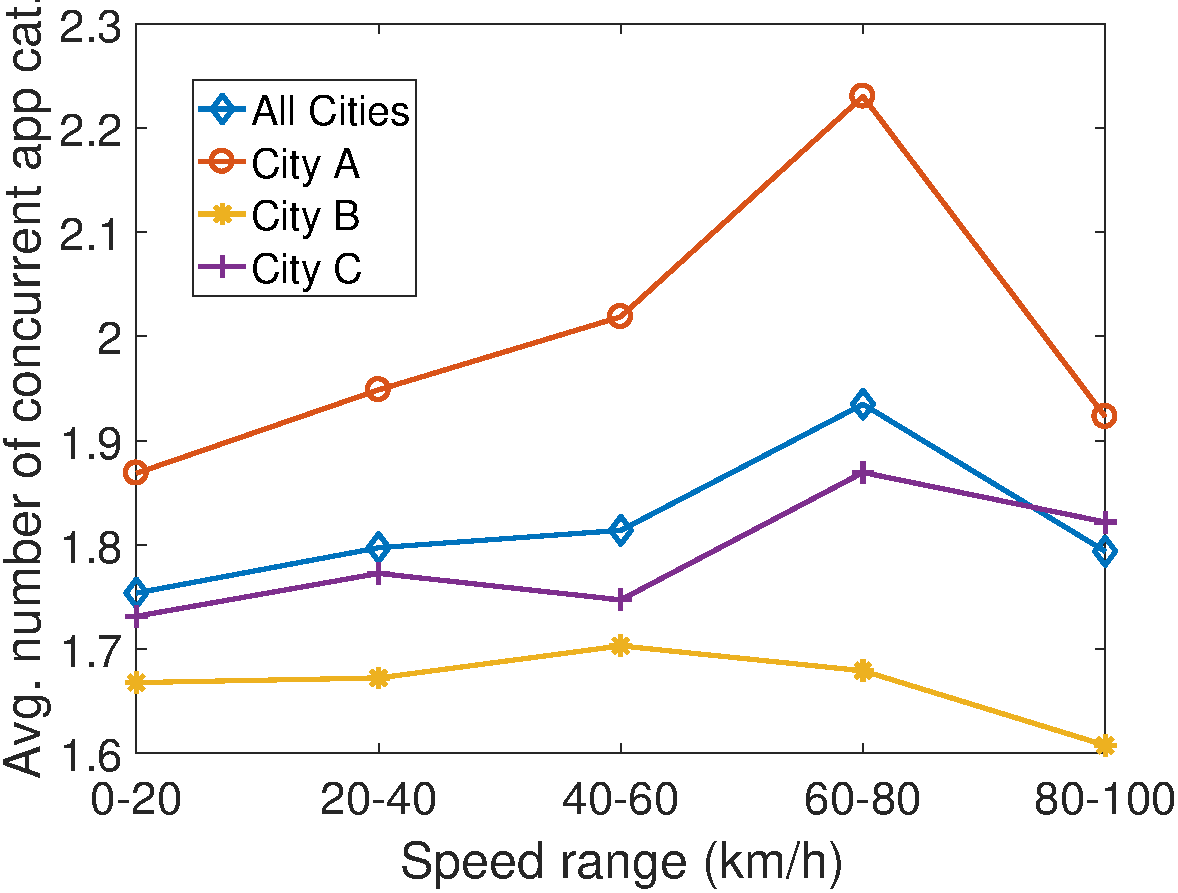
\includegraphics[width=0.48\linewidth]{./figures/app_category_overlap_8_6.pdf}}
    \caption{Correlation of user speed and the number of concurrently running apps and app categories}
    \label{fig:speed_concurrent_apps}
\end{figure*}
\end{comment}

We then further extended our study by investigating the correlation of the number of concurrently running apps and app categories with estimated user speed. The results are shown in \autoref{fig:app_overlap} and \autoref{fig:app_category_overlap}. %\autoref{fig:speed_concurrent_apps}. 
Although the actual launch time and closing time for each running app are unavailable, we use the network access data to infer such information. For each app, we treat the time of the first data access as the launch time of an app. If the app stops accessing network for a certain period (referred to as the closing threshold), we record the last network access time as the closing time for the app. We chose 10 seconds as the closing threshold to plot
%\autoref{fig:speed_concurrent_apps}, 
\autoref{fig:app_overlap} and \autoref{fig:app_category_overlap}, 
but we had tested various other thresholds and found similar trends. Interestingly, in most cities, the peak happens at the 60-80 km/h and decreases as the speed further increases. 

%\subsubsection{App Category Information}

%In this section,
Finally, we further investigated the trend of the contribution of various app categories on the total mobile data access as the user speed increases.
The contribution was defined as the mobile data access of one category versus all categories.
%However, the volume of data for each category is not even, among all 19 categories, we only interested in the
Focusing on apps that contributed the most to the total mobile data access volume,
we selected the top 8 app categories.
The correlation between the user speed and the contribution of each category is shown in \autoref{fig:speed_appcat}.
%Note that we do not show the correlation for each individual city because for some app categories there is not sufficient data to show a clear trend.

%\subsubsection{Impact of speed on each smartphone app category}

\begin{figure}[h]
    \centering
    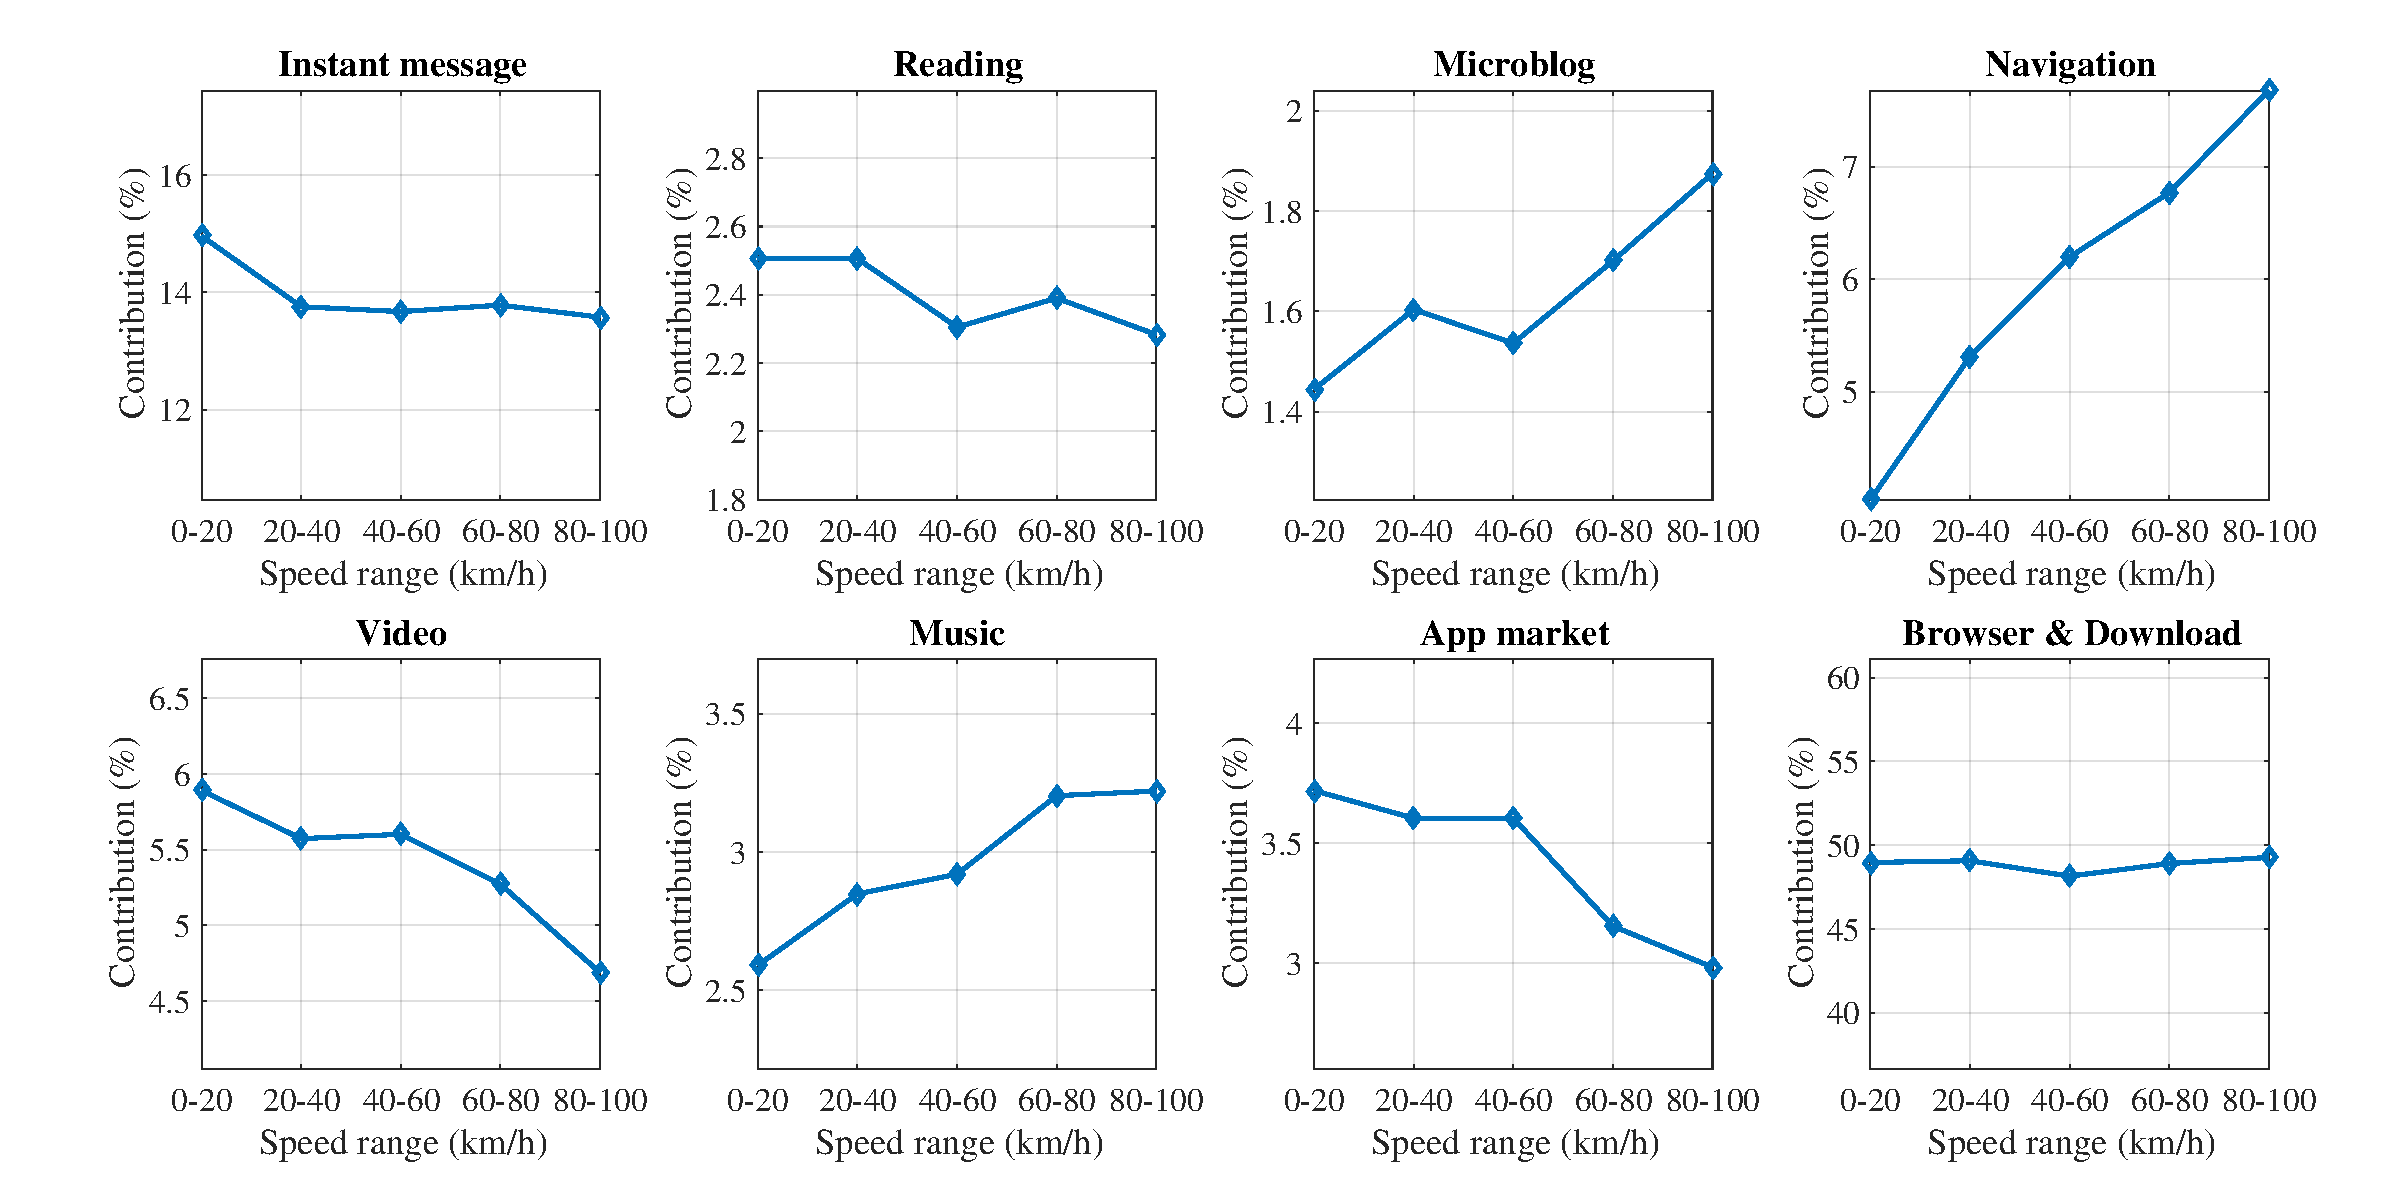
\includegraphics[width=\linewidth,height=3in]{./figures/large_font/speed_appcat.pdf}
    \vspace{-0.3in}
    \caption{Correlation of user speed and contribution of app categories.}
    \label{fig:speed_appcat}
\end{figure}

Among the top 8 categories, the Microblog, Navigation and Music categories show a clear upward trend as the speed increases.
The impact of navigation has the most steady increase due to the increased needs for such apps when driving.
The impact almost doubles for users with speed estimates of 80-100 km/h compared to users with speed estimates of 0-20 km/h.
Instant message, Video and App market show a downward trend as the speed increases.
The reason could be the users are cost sensitive and strictly control the data usage for large app downloading and video streaming.
Browser \& Downloading and Reading show a quite stable impact that does not change a lot as the speed increases.







